\subsubsection{Computing Geometric Affinity}\label{sec:curvGeod}
Affinities (or distances) between regions of the scene can be
computed as functions of the nodes of this mesh.
Following standard geometric mesh segmentation schemes
(\cite{Chen:2009:ABF, AZCXT11, lafarge2010})
we use surface curvature
as a heuristic for partitioning contiguous mesh regions.
In particular, we try to cut the mesh at ``creases'', regions where one of 
the principal curvature directions dominates the other.
At each mesh node, we compute the local principal curvatures $k_1(q)>k_2(q)$, and the corresponding 
principal directions $v_1(q)$ and $v_2(q)$, by fitting a second-order surface to that node and its neighbors.
The scalar field $K(q) := \max\{0, \frac{k_1(q)^2}{k_1(q) + |k_2(q)|}\}$ computed at every mesh node measures the strength and
dominance of the most-positive eigenvalue, $k_1(q)$ (see Figure \ref{fig:concavity}).
The augmented geometric distance between two points $q_i$ and $q_j$ on the mesh is computed as a $K$-weighted mesh geodesic,
that is, as the minimum path length $d_G(q_i,q_j) =  \min_{\left\{\substack{s_0\,\rightarrow\,\cdots\,\rightarrow\,s_n\\ q_i=s_0,\;q_j=s_n}\right\}}d_G(s_0,\ldots,s_n)$, where the $s_0,\ldots,s_n$ are a sequence of connected intervening nodes, $\{A_1, A_2\}$ are scalar weights, and
\begin{align}
%&\underset{\mathllap{\text{Geometric distance along path $s_0,\ldots,s_n$}}}{\underbrace{d_G(s_0,\ldots,s_n)}} 
&d_G(s_0,\ldots,s_n) 
\;:=\; \sum\nolimits_{i=1}^{n}\Bigl(\underset{\text{Path length}}{\underbrace{\|s_i-s_{i-1}\|_2}} \notag \\
&\qquad \;+\; 
\underset{\text{Concavity weight}}{\underbrace{K(s_i)}}\bigl(A_1\,
+\,A_2\underset{\mathclap{\text{Path-component in direction of greatest concavity\qquad}}}{\underbrace{|(s_i-s_{i-1})\cdot v_1(s_i)|}}\bigr)\Bigr) 
%\underset{\text{Concavity weight}}{\underbrace{\max\bigl\{0,\tfrac{k_1^2}{k_1+|k_2|}\bigr\}}}\bigl(A_1\,
%+\,A_2\underset{\mathclap{\text{Path along direction of greatest concavity\qquad\qquad}}}{\underbrace{|(s_i-s_{i-1})\cdot v_1|}}\bigr)\Bigr) 
\label{eq:dg}
\end{align}
A segmentation of the scene using these geometric homogeneity cues is a standard approach to 3D mesh segmentation, and is used as a baseline with which to evaluate our scale-aware segmentation in Sec. \ref{sec:evaluation}. A drawback of a purely geometric approach
is that there is no unique scale appropriate for a task-relevant segmentation (such as segmenting potential objects for manipulation), as 
scenes typically consist of multiple scales of geometric primitives with strong violations of homogeneity between them (think of a coffee mug or a pineapple).

 \begin{figure}
  \centering
 \begin{tabular}{cc}
 \includegraphics[width=0.45\textwidth]{figs/concavity.pdf}\qquad
 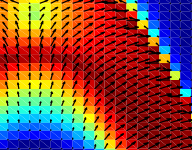
\includegraphics[width=0.45\textwidth]{figs/concavity_vectors.pdf}
 \end{tabular}

 \caption{\small Illustration of curvature penalty.  Paths are penalized
 which pass over regions with high concavity, especially in the direction of greatest concavity.
 At left, we show the scalar field $K(q)=\max\{0,k_1(q)^2/(k_1(q)+|k_2(q)|)\}$, on a sample curved surface, 
 where $k_1(q)$ is the greatest positive
 principal curvature component, with associated vector field $v_1(q)$.  
 At right, we show the weighted field $K(q)v_1(q)$ at each point.
 }\label{fig:concavity}
\vspace{-0.2in}
 \end{figure}
%-------------------------------------------------------------------------
\subsection{Constructing an Occlusion-Informed Geometry}\label{sec:geomOfObjs}
To upgrade this curvature-augmented geometry to one capable of supporting queries beyond geometric homogeneity, trained
detectors are typically used (e.g. \cite{haene2013, kundu2014}) to provide
semantic homogeneity cues. In lieu of a battery of
trained detectors for a fixed set of object classes, we obtain cues of topological characteristics \emph{as seen by the viewer} through occlusions
and use these to adapt the granularity of the distances on the scene to one relevant to the viewer's motion relative to the scene.
%-------------------------------------------------------------------------
\subsubsection{Single Image Occlusion-Based Segmentation}\label{sec:signatures}
Salient occlusion boundaries provide a strong topological cue as to the arrangement of surfaces in
the scene from a given vantage point and motion. Furthermore, they are derived from the measurements entirely at
runtime and not dependent on prior training data. We implement the linear program formulation of
\cite{ayvaciS12PAMI}, which employs occlusion relationships between regions on the image plane as
constraints on a depth-ordering of the image based on low level photometric
or geometric homogeneity cues.
Occlusion boundaries are obtained from salient depth discontinuities using the known geometry
of the scene, and the segmentation is performed on a superpixelization of the image derived from
the projected areas spanned by voxels associated to nodes of the scene mesh. These nodes are
coarsified based on proximity to generate a computationally tractable number of superpixels which
respect geometric boundaries in the images. Affinities between neighboring superpixels are found by
computing the cost $d_G$ between their corresponding nodes. Sample single
image segmentations are shown in section \ref{sec:results}.
Since the presence of salient occlusion cues is dependent on the viewpoint (and motion) of the camera, 
the back-projections of these segmentations give us a homogeneity cue \emph{relevant to the viewer's motion} to combine 
with the geometric homogeneity cues of Sec. \ref{sec:curvGeod}. To use these image segmentations $c_t$ as topological 
homogeneity cues, we aggregate a history $C(q) = \{C_t(q)\}_{t=1}^T$ at each node $q$. If the node $q$ is visible
in the image at time $t$, then $C_t(q)$ takes the mode of assignments in $c_t$ corresponding to the area its voxel subtends on the image plane. Zeroes in the history $C(q)$ denote frames in which the point $p$ is not visible.
A key assumption is that segmented regions in the images will be spatially consistent when
back-projected onto the scene. If they consistently have disagreeing 
labels, then they were typically considered to occupy different depth-layers from the viewer's perspective and are likely not part of the same region. 
We quantify this by accumulating a penalty $d_L$ along traversals of the scene that cross consistent image segmentation boundaries.
This penalty is the normalized total number of frames for which
the segmentation assignment changes, at least once, along the path (Eq. \ref{eq:dl}), 
as illustrated
in Fig. \ref{fig:layerPenalty}.
%\begin{align}
%&d_L(s_0,\ldots,s_n) :=\max_{i=1,\ldots,n} \notag\\
%&\quad \underset{\text{Fraction of frames in which $s_i$ is visible }}{\underbrace{\left\{
%\frac{|\{t\in 1,\ldots, T\;:\;0\neq c_t(s_j)\neq c_t(s_i)\neq 0,\;\exists j<i\}|}
%{N_0 + |\{t\in 1,\ldots, T\;:\;c_t(s_i)\neq 0\}|}
%\right\}}
%\label{eq:dl}
%\end{align}
\begin{align}
&d_L(s_0,\ldots,s_n) := \notag \\
%&\quad :=\max_{i=1,\ldots,n} \Biggl\{\frac{1}{N_0 + 
%\underset{\text{Frames in which $s_i$ is visible}}
%{\underbrace{|\{t\in 1,\ldots, T\;:\;c_t(s_i)\neq 0\}|}}}\notag\\
%&\quad \cdot
&\quad\tfrac{1}{T}
\underset{\mathclap{\text{Frames in which the layer assignment changes between $s_0$ and $s_n$}}}
{\underbrace{|\{t\;:\;\exists i,j\in 0,\ldots n,\;
0\neq C_t(s_j)\neq C_t(s_i)\neq 0\}|}}
\label{eq:dl}
\end{align}
Note that $0\leq d_L\leq 1$. 
%\FloatBarrier

\begin{figure}
    \centering
    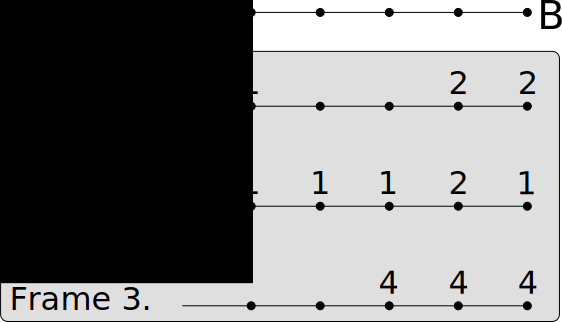
\includegraphics[width=0.45\linewidth]{figs/layer_histories.pdf}\qquad
    \includegraphics[width=0.45\linewidth]{figs/traversed_distances.pdf}
    \caption{\small At left, example back-projected image segmentation labels $c_t$ from three frames, over a sequence of nodes traversed from `A' to `B'. At right, the traversal penalty $d_L$ accumulated over the traversal due to passing through nodes with conflicting image segmentation histories. The fact that some nodes are not visible in some frames means that penalties are not
    incurred along the same boundaries, depending on the direction of travel.}
\label{fig:layerPenalty}

\end{figure}


%-------------------------------------------------------------------------
\subsubsection{Occlusion-Constrained Geometric Affinity}\label{sec:adaptiveGeo}
Secs. \ref{sec:curvGeod} and \ref{sec:signatures} present two different traversal costs along the nodes of the mesh.
$d_G$ models deviations from geometric homogeneity, and $d_L$ models violations of image topology informed by occlusions.
Nonparametric segmentation techniques (such as those used in Sec. \ref{sec:segmentation}) are preferred for generic segmentation
tasks due to their ability to select the number of segments automatically. As a consequence, any combination of $d_G$ and $d_L$ between
two nodes must change the structure of the resulting scene distance matrix at all scales in order to be effective. For example, a cost $d(q_i, q_j) = d_G(q_i, q_j)+d_L(q_i, q_j)$ will amplify geometric distances linearly when $d_L(q_i, q_j) \neq 0$, and have no impact on distances within
contiguous regions bounded by occlusions cues in the images. This will likely lead to over-segmentations of the scene in those regions when using non-parametric methods. 
Therefore a key design criterion for our adaptation of the geometric costs $d_G$ between nodes using $d_L$ is that they be \emph{attenuated} when $d_L$ is small and \emph{amplified} when $d_L$ is close to one.

To achieve this, and serve the dual purpose of providing a natural conversion from distances $d_G$ to affinities for segmentation, we compute the cost of traversing a path between successive adjacent nodes on the scene using the Geman-McClure robust penalty (Eq. \ref{eq:geman_mcclure}) with a scale parameter $\sigma_{\alpha,\eps}(d_L)$ (Eq. \ref{eq:shaping}).
\begin{equation}
d(q_i, q_j) = \min_{\left\{\substack{s_0\,\rightarrow\,\cdots\,\rightarrow\,s_n\\ q_i=s_0,\;q_j=s_n}\right\}}
\left(1+\frac{\sigma_{\alpha,\eps} (d_L(s_0,\ldots,s_n))^2}{d_G(s_0,\ldots,s_n)^2}\right)^{-1},
\label{eq:geman_mcclure}
\end{equation}
$\sigma_{\alpha,\eps}(d_L)$ acts as a \emph{scale shaping} function, the goal of which is to locally adapt the scale of the distance function based on
the available evidence for object boundaries. If minimal evidence is present ($d_L$ is small),
$\sigma_{\alpha,\eps}$ will be large and attenuate the increase in distance. If $d_L$ is large and
a consistent boundary in back-projected image segmentations is present then $\sigma_{\alpha,\eps}(d_L)$
will shrink, accelerating the increase in distance. The parameters $\alpha$ and $\eps$ control the rate of decreasing scale and boundary values (at $d_L=0$ and $d_L=1$) respectively. Fig. \ref{fig:shapingFn} shows an example of the behavior of this choice of combined geodesic and adaptive scale using artificial data.

% \begin{equation}\label{eq:dg}
% \begin{split}
%  d_G(s_0,\ldots,s_n) = \sum\nolimits_{i=1}^{n}\Bigl(\|s_i-s_{i-1}\|_2 + \\
% \max\bigl\{0,\tfrac{k_1^2}{k_1+|k_2|}\bigr\}\bigl(A_1\,+\,A_2|(s_i-s_{i-1})\cdot v_1|\bigr)\Bigr)
% \end{split}
% \end{equation}
% 
% \begin{equation}\label{eq:dl}
% \begin{split}nv
% d_L(s_0,\ldots,s_n) = \\ \tfrac{1}{n}\bigl|\bigl\{j\,:\,0 \neq c_{t_j}(s_{k}) \neq
% c_{t_j}(s_{\ell})\neq0,\quad \\
% \text{for some $k,\ell$ in $0,\ldots,n$}\bigr\}\bigr|.
% \end{split}
% \end{equation}

\begin{equation}\label{eq:shaping}
\sigma_{\alpha,\eps}(d_L) = \frac{1-\exp(-\alpha(1-d_L)-\eps)}{1-\exp(-d_L-\eps)}
\end{equation}
\begin{figure}
    \centering
    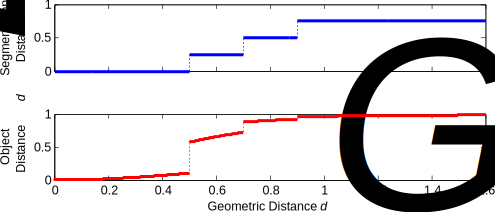
\includegraphics[width=0.95\linewidth]{figs/saturating_distances}
    \caption{\small Example behavior of the combined traversal cost in Eq. \ref{eq:geman_mcclure} using artificial data.
    Note that as $d_L$ increases, the rate of increase of $d$ as a function of $d_G$ accelerates up until saturation of the robust penalty.}
\label{fig:shapingFn}

\end{figure}


The set of distances $d_i := \{d_{ij}\;:\;j\in S\}$ is computed in $O(|S|\,n_{\text{frames}})$ time,
using a modified Dijkstra's algorithm on the nodes of the scene mesh.

%%\FloatBarrier
%
%\begin{figure*}
%\begin{equation}
%\smash{
%\underset{\mathclap{\text{Geometric distance along path $s_0,\ldots,s_n$}}}{\underbrace{d_G(s_0,\ldots,s_n)}} 
%\;=\; \sum\nolimits_{i=1}^{n}\Bigl(\underset{\text{Path length}}{\underbrace{\|s_i-s_{i-1}\|_2}} \;+\;
%\underset{\text{Concavity weight}}{\underbrace{\max\bigl\{0,\tfrac{k_1^2}{k_1+|k_2|}\bigr\}}}\bigl(A_1\,
%+\,A_2\underset{\mathclap{\text{Path comp. in direction of greatest concavity}}}{\underbrace{|(s_i-s_{i-1})\cdot v_1|}}\bigr)\Bigr)\\
%}
%\label{eq:dg}
%\end{equation}
%\begin{equation}
%\smash{
%\underset{\mathclap{\text{Layer distance along path $s_0,\ldots,s_n$}}}{\underbrace{d_L(s_0,\ldots,s_n)}} 
%\;=\; \tfrac{1}{n}\,
%\underset{\text{Number of changes between nonzero layer assignments}}
%{\underbrace{\max\bigl\{|\{0\leq i_1<\ldots<i_k\leq n\}|\;:\; 0\neq c(s_{i_{\ell}})\neq c(s_{i_{\ell+1}})\neq0,\; \forall\;\ell=1,\ldots,k-1\bigr\}}}
%}
%\label{eq:dl}
%\end{equation}
%%\begin{caption}{Path-length components}
%%Path-length on the mesh is computed as a com
%%\end{caption}
%\end{figure*}
%\addtocounter{enumi}{-1}
%%\FloatBarrier

\begin{figure}
\begin{center}
  \centerline
      {
        \hbox
            {%\\
              \begin{tabular}{cc}
		{\includegraphics[width=0.45\textwidth]{figs/cos/geotrav.png}}
		{\includegraphics[width=0.45\textwidth]{figs/park4/geotrav.png}}
		\\
		{\includegraphics[width=0.45\textwidth]{figs/pipes2/geotrav.png}}
		{\includegraphics[width=0.45\textwidth]{figs/pipes3/geotrav.png}}
              \end{tabular}
            }
      }
\end{center}
   \caption{\small Sample geometric traversal costs $d_G$ from a single point to all others across the scene overlaid on images.
Colored lines indicate the path of the geodesic on the scene originating at the magenta square in each image, with distance increasing with changing colors, starting from zero (black).}
\label{fig:geoTravs}
\end{figure}

%-------------------------------------------------------------------------
\subsection{Scene Segmentation}\label{sec:segmentation}
Discrete
representations of complex scenes at high resolution can typically consist of many thousands of
nodes, making both computation and storage of a pairwise distance matrix of geodesics between all nodes infeasible. To make
segmentation based on pairwise distances tractable we generate a subgraph of the scene by
uniformly sampling nodes subject to a minimum Euclidean distance and compute geodesics
between them using the full resolution representation. To obtain a sparse segmentation of the scene, we apply a graph-based version of the
DP-Means~\cite{Kulis12_ICML} algorithm, a low-variance asymptotic clustering algorithm derived from
the Dirichlet process Gaussian mixture model~\cite{Teh10_EML}. The DP-Means algorithm was chosen for
its nonparametric nature, i.e.~its ability to select the number of objects in the scene
automatically, and its computational speed. However, the original algorithm is only applicable to
clustering data in a normed vector space; thus, we find an initial segmentation of the
subgraph by globally optimizing a spectral relaxation~\cite{Zha01_NIPS,Yu03_ICCV} of the DP-Means
cost, and refine the segmentation via kernelized~\cite{Dhillon07_TPAMI} iterative
updates. The partitioned subgraph is projected back to full mesh by performing a Voronoi
tessellation of the scene discretization using the previously computed geodesics from each node in the subgraph.

A possible future extension of our segmentation pipeline is to enable adaptation to dynamically changing scales by treating more recent images segmentations preferentially, either through a fixed sliding window or decaying components of  $d_L(s_0,\ldots,s_n)$. The Dynamic Means~\cite{Campbell13_NIPS} algorithm, a low-variance
asymptotic clustering algorithm based on the dependent Dirichlet process Gaussian
mixture~\cite{Lin10_NIPS} can be used to make such a segmentation strategy temporally consistent. As in the batch case, this algorithm is ideal due
its nonparametric ability to automatically discover the number of objects in the
scene, and for its computational speed. However, Dynamic Means suffers from the
same limitation as DP-Means; it is only applicable to data in a normed vector
space. Therefore, for each video frame, we find an initial segmentation of the
single frame alone using spectral clustering, and then enforce temporal consistency in the
segmentation by using kernelized refinement iterations based on the Dynamic Means cost.
